\chapter*{Приложение А}
\addcontentsline{toc}{chapter}{Приложение А}

Приложение содержит UML диаграмму классов архитектурного домена.

\begin{figure}
	\centering
	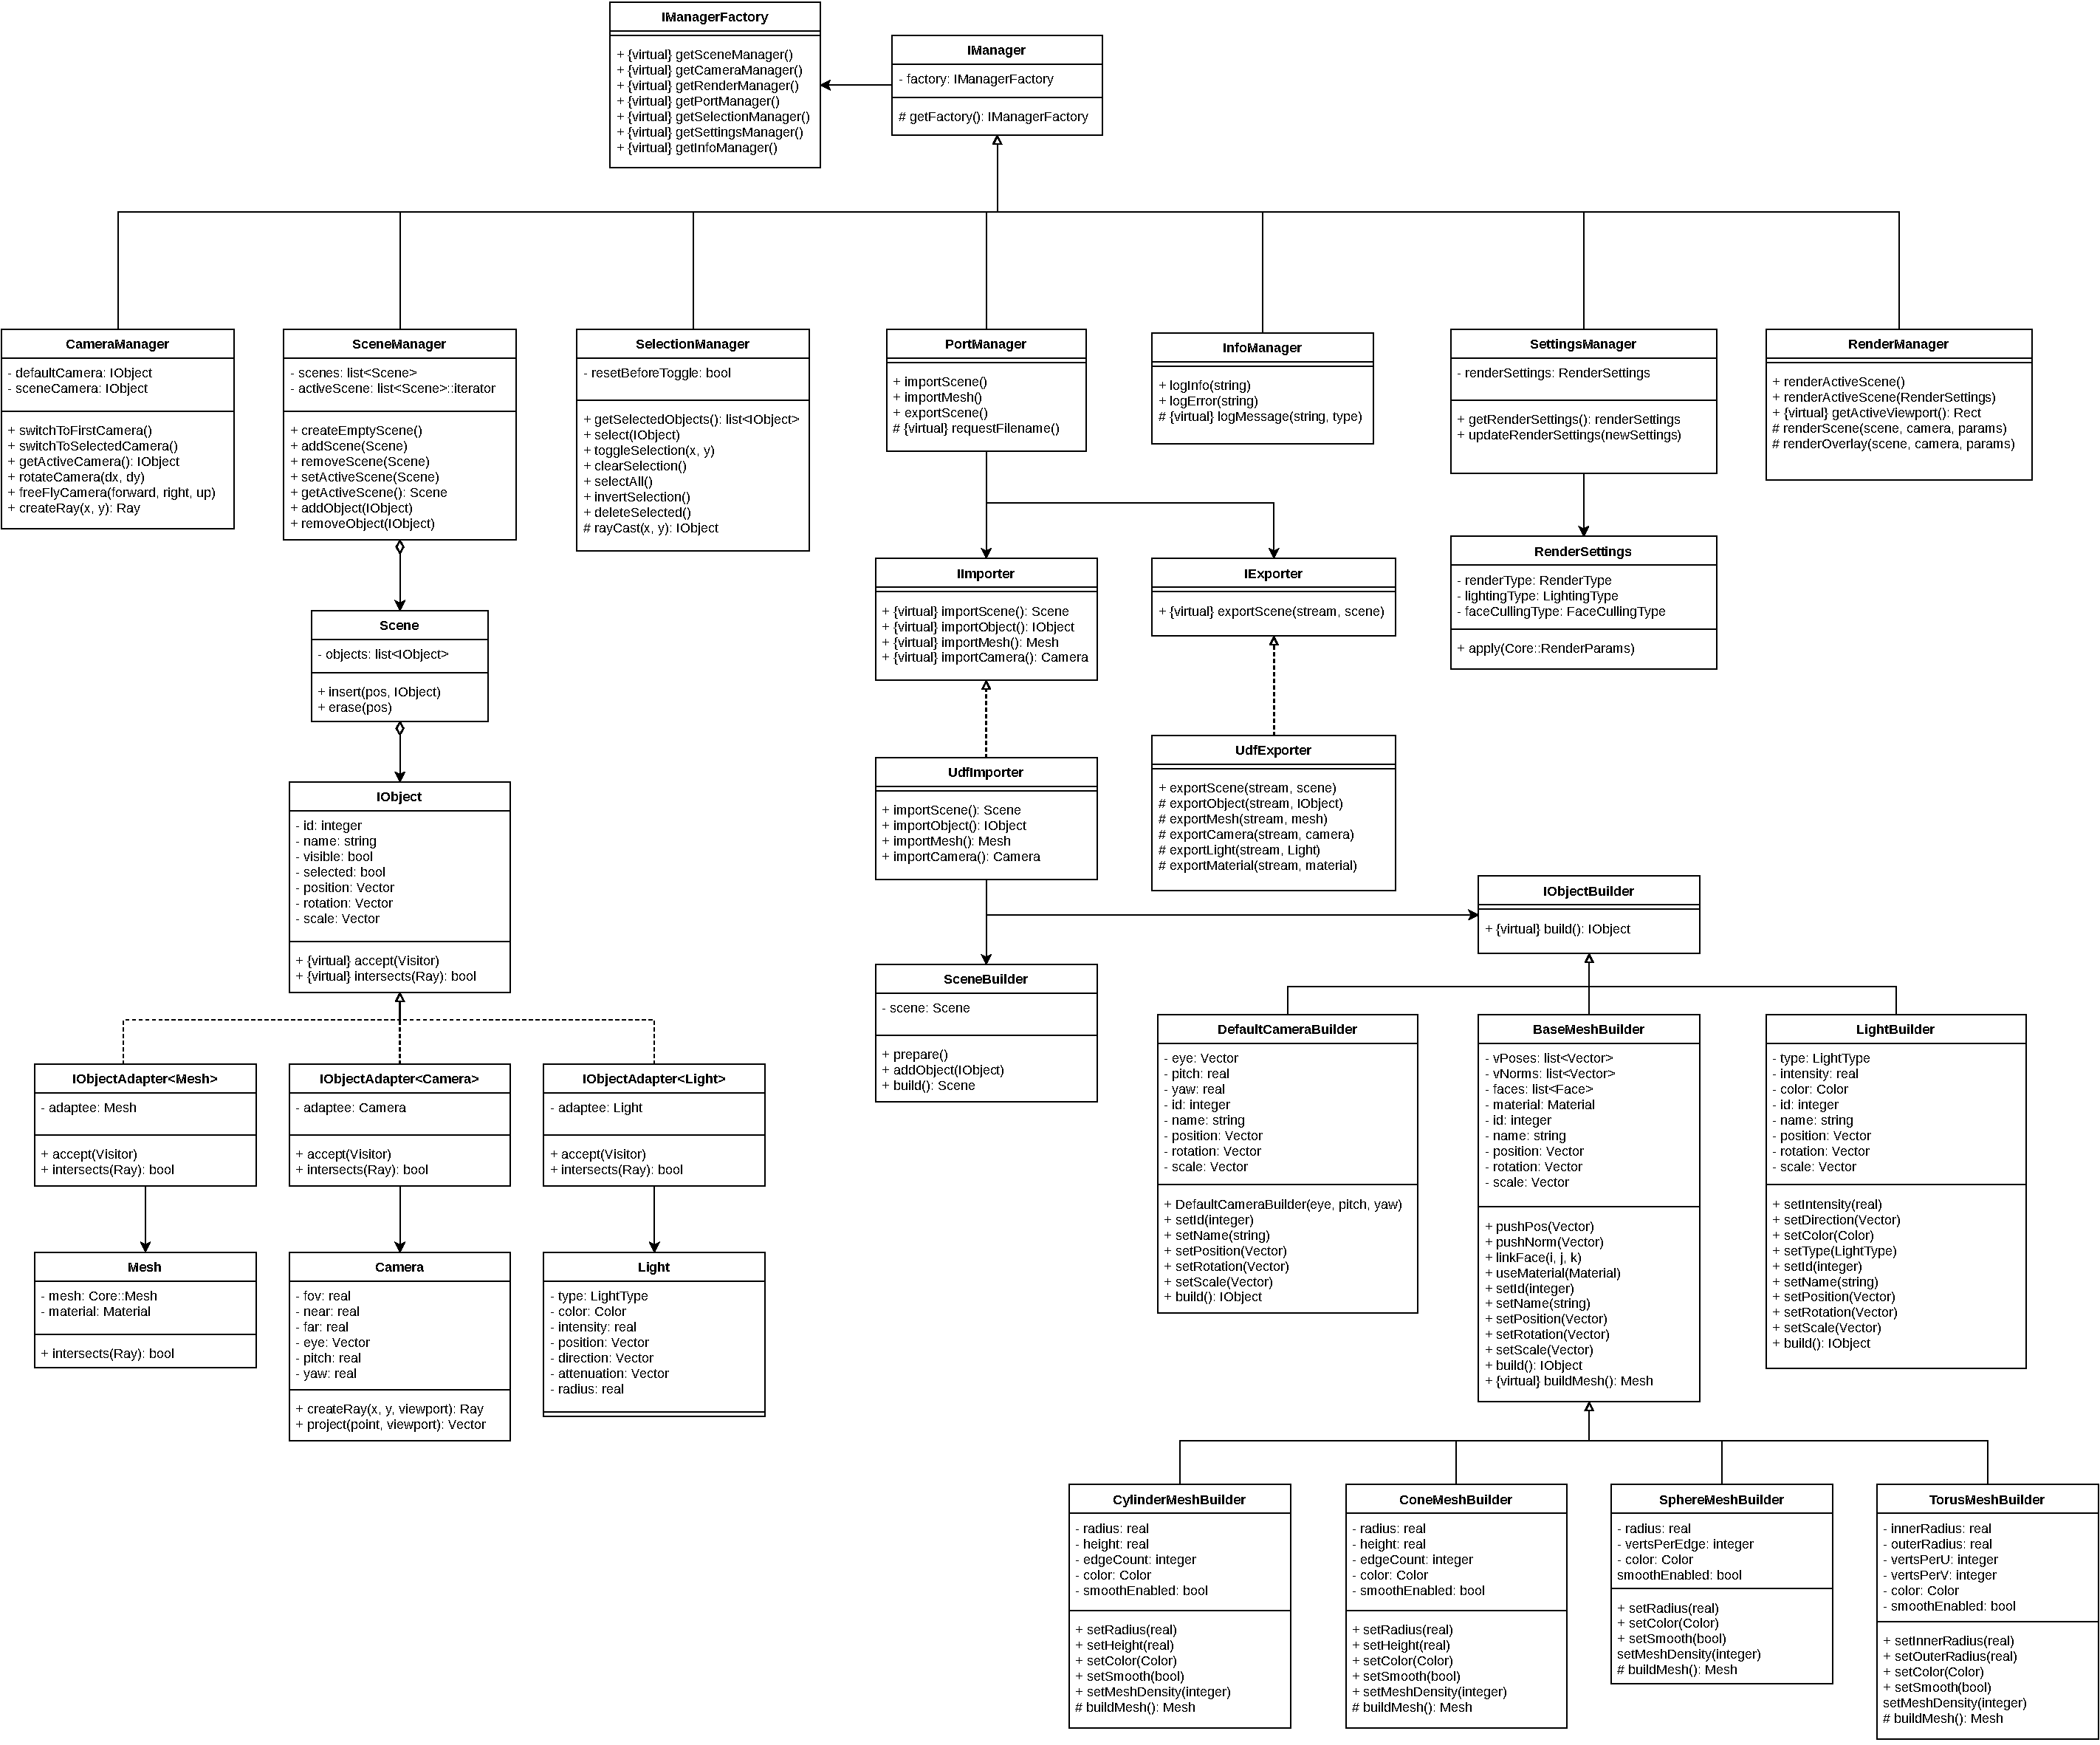
\includegraphics[angle=90,width=\linewidth,height=\textheight,keepaspectratio]{diagrams/uml.pdf}
	\caption{UML диаграмма классов архитектурного домена}
	\label{uml:arch}
\end{figure}

\chapter*{Приложение Б}
\addcontentsline{toc}{chapter}{Приложение Б}

Приложение содержит скриншоты интерфейса программного продукта.

\begin{figure}
	\centering
	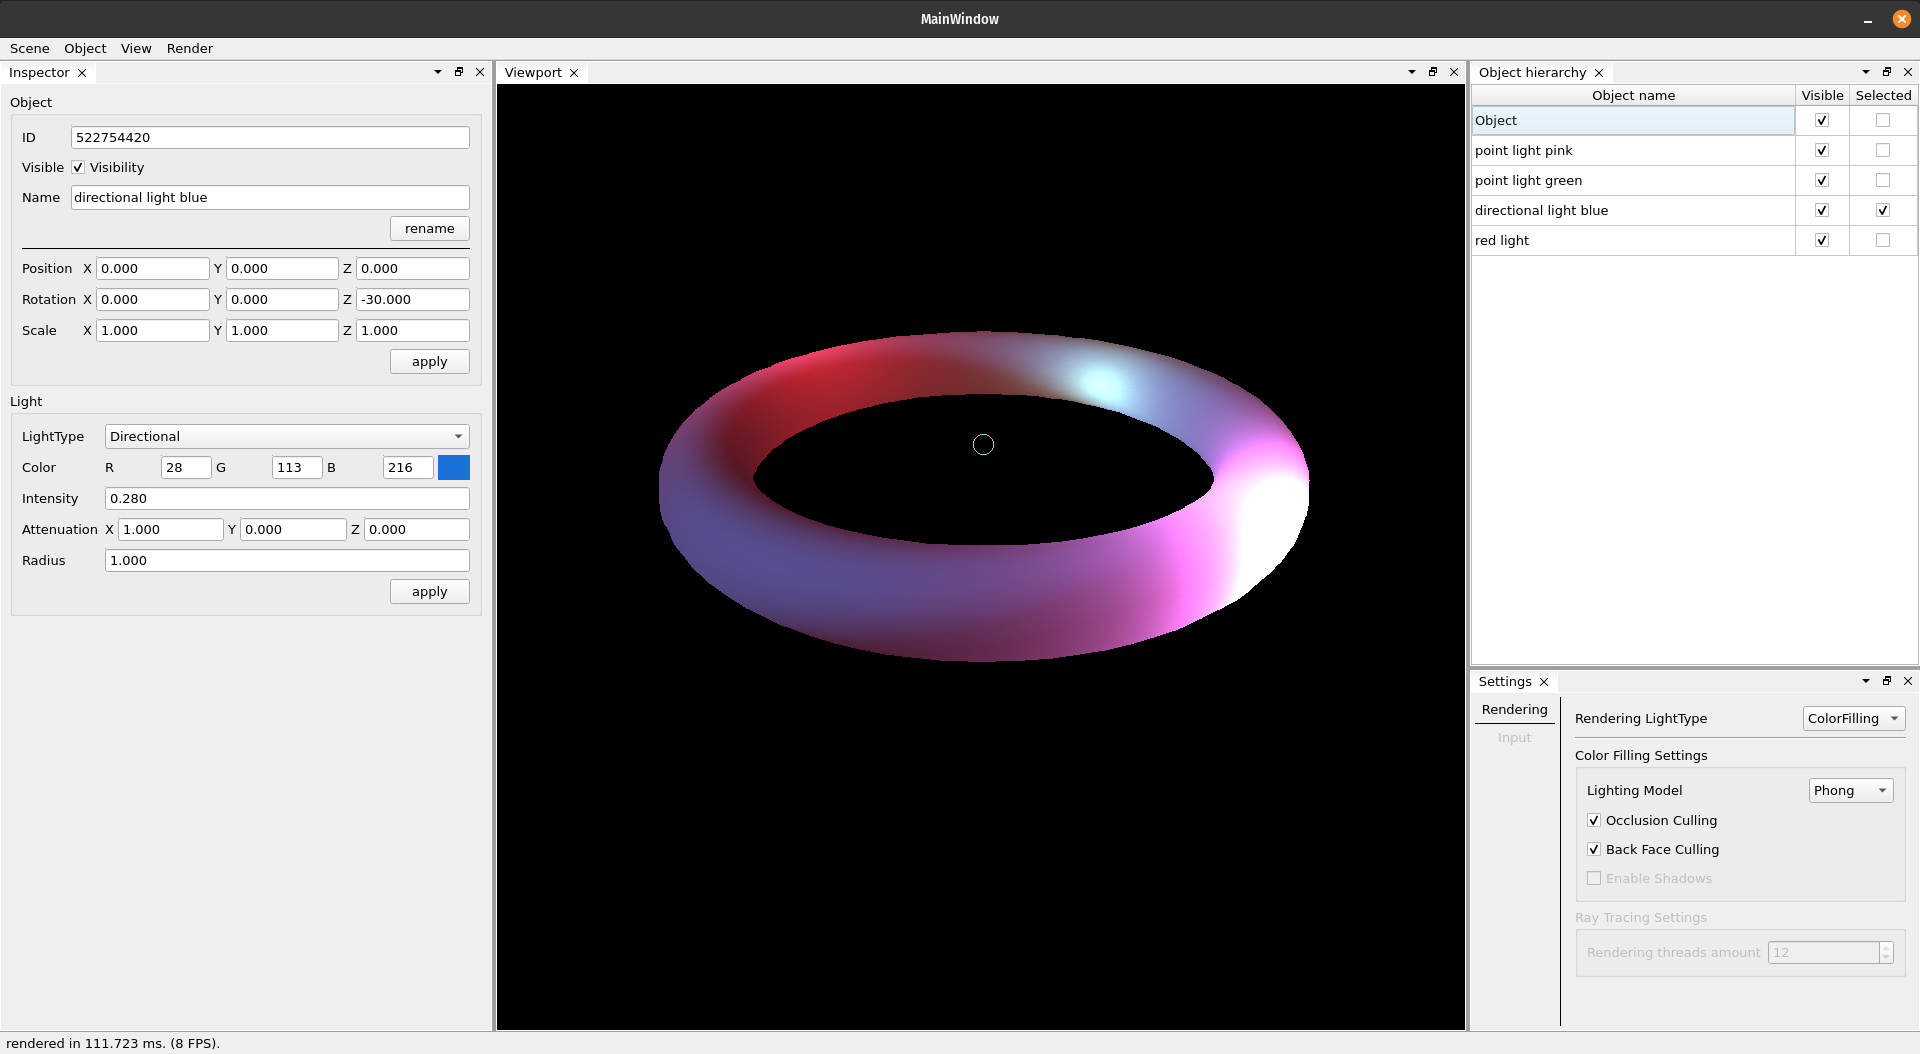
\includegraphics[angle=90,origin=c,width=\linewidth,height=0.7\textheight,keepaspectratio]{inc/img/screenshot-1.png}
	\caption{Интерфейс программы}
	\label{demo:screenshot:1}
\end{figure}

\begin{figure}
	\centering
	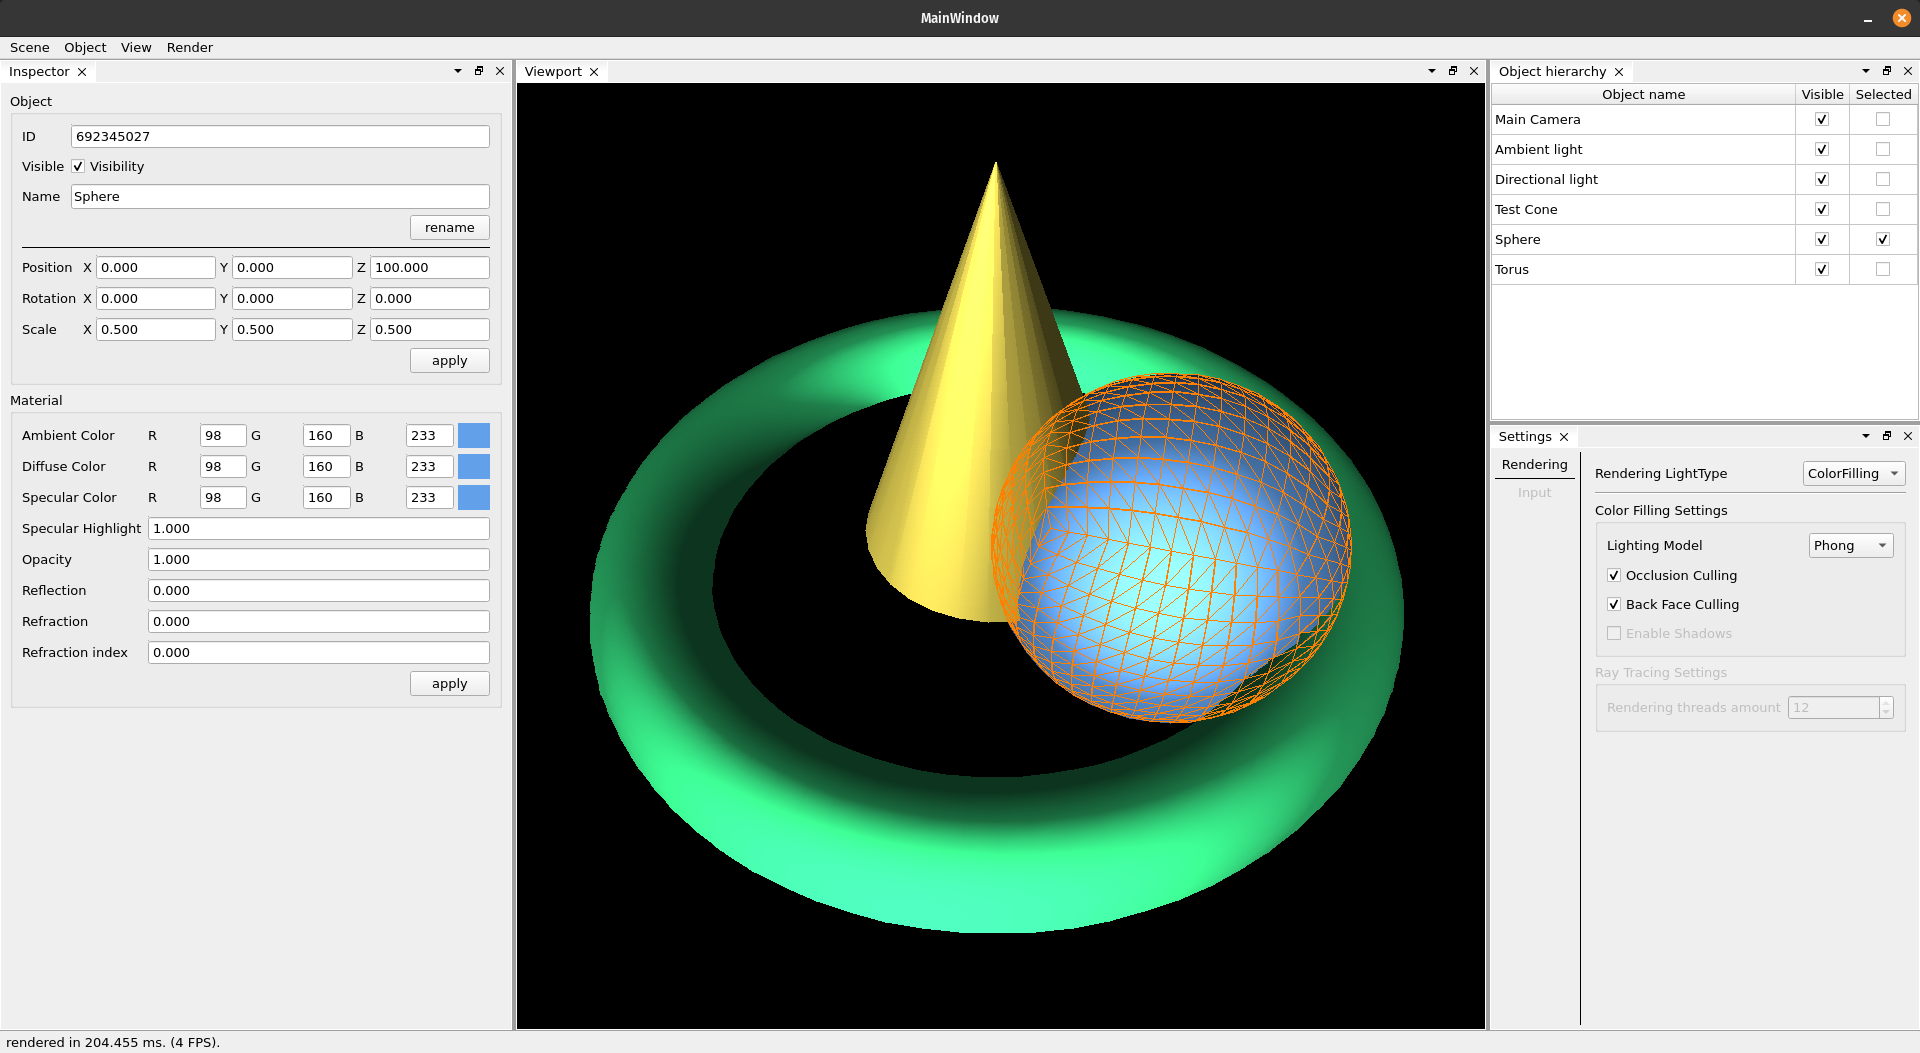
\includegraphics[angle=90,origin=c,width=\linewidth,height=0.7\textheight,keepaspectratio]{inc/img/screenshot-2.png}
	\caption{Редактирование параметров объекта сцены}
	\label{demo:screenshot:2}
\end{figure}

\begin{figure}
	\centering
	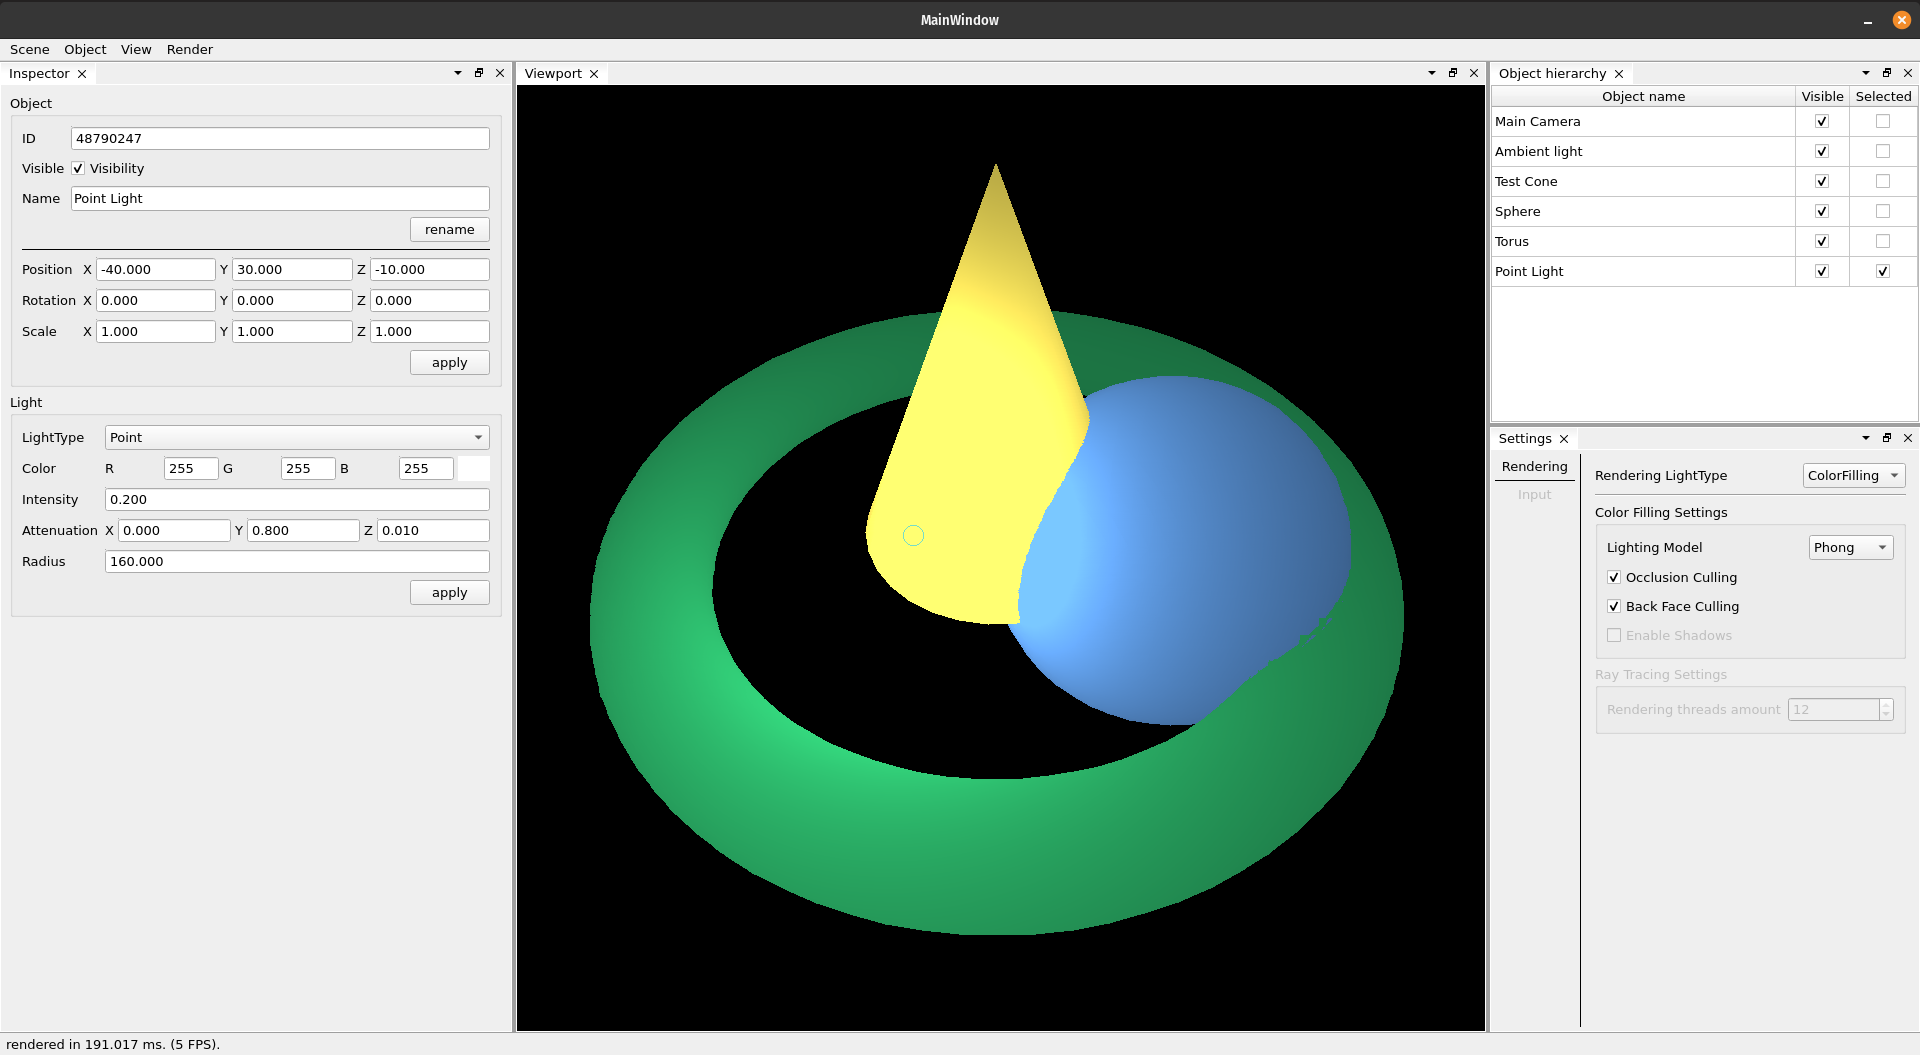
\includegraphics[angle=90,origin=c,width=\linewidth,height=0.7\textheight,keepaspectratio]{inc/img/screenshot-3.png}
	\caption{Смена направленного освещения на точечное}
	\label{demo:screenshot:3}
\end{figure}